\documentclass[handout]{beamer}

\usetheme[progressbar=frametitle]{metropolis}
\metroset{block=fill}

\subtitle{NTIN071 Automata and Grammars}
\author{Jakub Bulín (KTIML MFF UK)}

\date{Spring 2025\\ 
    \vspace{1in} 
    \begin{flushleft}
        \it \footnotesize * Adapted from the Czech-lecture slides by Marta Vomlelová with gratitude. The translation, some modifications, and all errors are mine.
    \end{flushleft}
}

%% packages

\usepackage{amsmath}
\usepackage{amssymb}
\usepackage{amsthm}
\usepackage{cancel}
\usepackage{color}
\usepackage{colortbl}
\usepackage{forest}
\usepackage[utf8x]{inputenc}
\usepackage{multicol}
\usepackage{multirow}

%% colors
\definecolor{Gray}{gray}{0.9}

%% TikZ
\usepackage{tikz}
    \usetikzlibrary{
        automata,
        arrows,
        backgrounds,
        decorations.pathmorphing,
        fit,
        positioning,
        shapes,
        shapes.geometric,
        tikzmark
    } 
    \tikzset{>=stealth',shorten >=1pt,auto,node distance=2cm}
    \tikzset{initial text={}}
    \tikzset{elliptic state/.style={draw,ellipse}}

%% amsthm
\theoremstyle{plain}
    \newtheorem*{algorithm}{Algorithm}    
    \newtheorem*{observation}{Observation}
    \newtheorem*{proposition}{Proposition}

\theoremstyle{remark}
    \newtheorem*{exercise}{Exercise}
    \newtheorem*{remark}{Remark}

%% macros
\DeclareMathOperator{\RegE}{RegE}
\DeclareMathOperator{\RL}{RL}

% Just for Lecture 2
\newcommand{\x}{$\times$}
\newcommand{\nx}{\ }



\title{Lecture 5 -- Formal grammars, regular and context-free grammars}


\begin{document}


\frame{\titlepage}


\begin{frame}{Recap of Lecture 4}

    \begin{itemize}
        \item regular expressions
        \item Kleene's theorem (two variants)
        \item constructions: RE to $\epsilon$-NFA, DFA to RE
        \item state elimination algorithm
        \item string substitution, homomorphism, inverse homomorphism
        \item decision properties
    \end{itemize}

\end{frame}


\section{\sc Chapter 2: Grammars}


\section{2.1 Formal grammars}


\begin{frame}{Palindromes are not regular}

    \alert{palindrome}: $w=w^R$, e.g. \texttt{racecar}, \texttt{step\_on\_no\_pets}

    \begin{example}
        The language $L_\mathrm{pal}=\{w\in\{0,1\}^*\mid w=w^R\}$ is not regular.

        (A standard Pumping lemma argument using $w=0^n10^n$.)
    \end{example}    

    How to represent $L_\mathrm{pal}$? We can use a (\alert{context-free}) \alert{grammar},     
    $G=(\{S\},\{0,1\},\mathcal P,S)$ with the following set of \alert{production rules}:
    \begin{align*}
        \mathcal P=\{&S\rightarrow \epsilon,\\
        &S\rightarrow 0,\\
        &S\rightarrow 1,\\
        &S\rightarrow 0S0,\\
        &S\rightarrow 1S1\}
    \end{align*}
	For brevity, we also write $\mathcal P=\{S\rightarrow \epsilon\mid 0\mid 1\mid 0S0\mid 1S1\}$.

\end{frame}


\begin{frame}{Formal grammar: the definition}

    A \alert{formal (generative) grammar}: $G=(V,T,\mathcal P,S)$ where
    \begin{itemize}
        \item $V$ is a finite nonempty set of \alert{nonterminals} (\alert{variables})
        \item $T$ is a finite set of \alert{terminal symbols} (\alert{terminals}), $V\cap T=\emptyset$
        \item $S\in V$ is the \alert{start symbol}
        \item $\mathcal P$ is a finite set of \alert{production rules} of the form $\alpha\to\beta$ where 
		\begin{itemize}
			\item $\alpha\in(V\cup T)^+\setminus T^+$, the \alert{head} (must contain some variable!)
			\item $\beta\in(V\cup T)^*$, the \alert{body}
		\end{itemize}
    \end{itemize}

	A grammar is \alert{context-free} (a \alert{CFG}) if the head is a single variable, i.e., the rules are of the form $A\to\beta$ for $A\in V$ and $\beta\in(V\cup T)^*$.
    
	\bigskip

	The production rules thus represent a \alert{recursive definition of the language}, starting from the start symbol (see the example).	 

\end{frame}


\begin{frame}{Derivation, the language of a grammar}

	Let $G=(V,T,\mathcal P,S)$ be a grammar.
	\begin{itemize}
		\item $\gamma$ \alert{one-step derives} $\delta$ (write \alert{$\gamma\Rightarrow_G\delta$} or just \alert{$\gamma\Rightarrow\delta$}) if $\gamma=\eta\alpha\nu$ and $\delta=\eta\beta\nu$ for some $\alpha\to\beta\in\mathcal P$ and $\eta,\nu\in(V\cup T)^*$
		
		\item $\gamma$ \alert{derives} $\delta$ (write \alert{$\gamma\Rightarrow_G^*\delta$} or just \alert{$\gamma\Rightarrow^*\delta$}) if there are $\beta_1,\dots,\beta_n\in (V\cup T)^*$ s.t.
		$\gamma=\beta_1\Rightarrow\beta_2\Rightarrow\dots\Rightarrow\beta_n=\delta$\\
		(Note that always $\gamma\Rightarrow^*\gamma$.)

		\item the sequence $\beta_1,\dots,\beta_n$ is a \alert{derivation} of $\delta$ from $\gamma$, it is \alert{minimal} if $\beta_i\neq\beta_j$ for $i\neq j$
		\item a \alert{sentential form} is any $\delta\in(V\cup T)^*$ such that $S\Rightarrow_G^*\delta$		
	\end{itemize}

	The language \alert{generated by } $G$, \alert{$L(G)$} consists of words over the terminals derivable from the start symbol:
	\alert{$$
	L(G)=\{\omega\in T^*\mid S\Rightarrow^*_G \omega\}
	$$}
	(Similarly, for any $A\in V$ define $L(A)=\{\omega\in T^*\mid A\Rightarrow^*_G \omega\}$.)
	
\end{frame}


\section{2.2 Chomsky hierarchy}


\begin{frame}{Chomsky hierarchy (of grammars)}

	Restricting the form of production rules:

	\begin{itemize}
		\item Type 0: \textbf{general grammars}
		\begin{itemize}
			\item \alert{$\alpha_1 A \alpha_2\to\beta$} where $A\in V$, $\alpha_1,\alpha_2,\beta\in (V\cup T)^*$
			\item recursively enumerable languages ${\mathcal L}_0$
		\end{itemize}

		\medskip
		
		\item Type 1: \textbf{context-sensitive grammars}
		\begin{itemize}
			\item \alert{$\alpha_1 A \alpha_2\rightarrow \alpha_1\gamma\alpha_2$}, $A\in V$, $\gamma\in(V\cup T)^+$, $\alpha_1,\alpha_2\in (V\cup T)^*$
			\item note: the variable must be rewritten to at least one symbol
			\item sometimes we allow $S\to\epsilon$, then $S$ cannot appear in any body
			\item context-sensitive languages ${\mathcal L}_1$
		\end{itemize}
		
		\medskip

		\item Type 2: \textbf{context-free grammars}
		\begin{itemize}
			\item \alert{$A\to\beta$} where $A\in V$, $\beta\in (V\cup T)^*$
			\item context-free languages ${\mathcal L}_2$
		\end{itemize}

		\medskip

		\item Type 3: \textbf{right-linear grammars} (aka regular grammars)
		\begin{itemize}
			\item \alert{$A\to\omega B$} or \alert{$A\to\omega$} where $A,B\in V$, $\omega\in T^*$
			\item regular languages ${\mathcal L}_3$
		\end{itemize}
	
	\end{itemize}

\end{frame}


\begin{frame}{The classes are ordered by (strict) inclusion}

	\Huge{
		$$
		{\mathcal L}_0\supset {\mathcal L}_1 \supset {\mathcal L}_2\supset {\mathcal L}_3 
		$$
	}

	\bigskip

	\normalsize{

	\begin{itemize}
		\item context-sensitive languages are recursively enumerable: the head of a CSG contains a variable

		\item context-free languages are context-sensitive: the context $\alpha_1,\alpha_2$ is empty; we can \alert{eliminate $\epsilon$-productions} $A\to\epsilon$

		\item regular languages are context-free: body can have any form 

		\item strict inclusion: we will give examples later
	\end{itemize}

	}

\end{frame}


\section{2.3 Regular grammars}

\begin{frame}{Right-linear grammars}

	A grammar $G$ is \alert{right-linear} (\alert{regular}, \alert{type 3}), if its production rules are of the form \alert{$A\to\omega B$} or \alert{$A\to\omega$} where $A,B\in V$, $\omega\in T^*$.

	(At most one variable in the body, it can only be at the end.)

	\begin{example}
		$G=(\{S,A,B\},\{0,1\},\mathcal P,S)$ where
		
		\vspace{-12pt}
		$$
		\mathcal P=\{S\rightarrow 0S\mid 1A\mid \epsilon,\ A\rightarrow 0A\mid 1B,\ B\rightarrow 0B\mid 1S\}
		$$

		\vspace{-6pt}
		A derivation of $01101\in L(G)$:

		\vspace{-24pt}
		$$
		S\Rightarrow 0S\Rightarrow 01A \Rightarrow 011B \Rightarrow 0110B \Rightarrow 01101S \Rightarrow 01101
		$$
		
		\vspace{-6pt}
	\end{example}
	Corresponds to FA: nonterminals are states, generate means read.

	\begin{theorem}
		A language is regular, iff it is generated by a right-linear grammar.
	\end{theorem}

\end{frame}


\begin{frame}{Example: binary numbers divisible by 5}

	\begin{columns}

		\column{0.5\textwidth}

		\vspace{12pt}
		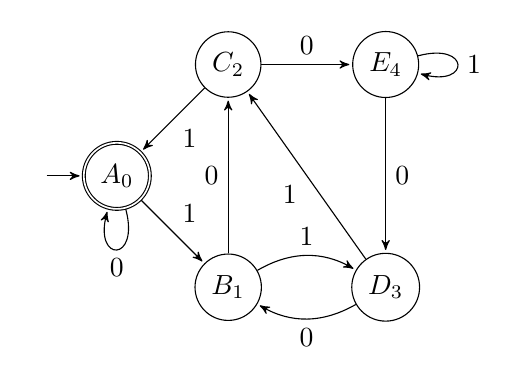
\begin{tikzpicture}[>=stealth',shorten >=1pt,auto,node distance=2cm]
			\tikzset{every state/.style={minimum size=0.2cm}}
			\node[initial,state,accepting] (a)      {$A_0$};
			\node[state] (b)  [below right of=a]     {$B_1$};
			\node[state] (c) [above right of=a]     {$C_2$};
			\node[state] (d) [right of=b]     {$D_3$};
			\node[state] [right of=c]   (e)   {$E_4$};
			\path[->]
				(a)  edge [loop below]  node {0} (a)
				(a)  edge  node {1} (b)
				(b)  edge node {0} (c)
				(b)  edge [bend left] node {1} (d)
				(c)  edge node {1} (a)
				(c)  edge  node {0} (e)
				(d)  edge [bend left] node {0} (b)
				(d)  edge  node {1} (c)
				(e)  edge [loop right] node {1} (e)
				(e)  edge  node {0} (d);
		\end{tikzpicture}	
	
		\column{0.5\textwidth}
		
		\vspace{-18pt}
		\begin{eqnarray*}
			A& \rightarrow & 1B\mid 0A\mid \epsilon\\
			B& \rightarrow & 0C\mid 1D\\
			C& \rightarrow & 0E\mid 1A\\
			D& \rightarrow & 0B\mid 1C\\
			E& \rightarrow & 0D\mid 1E
		\end{eqnarray*}
		
	\end{columns}

	\bigskip
	Derivation examples

	\begin{tabular}{l l}
		$A\Rightarrow 0A\Rightarrow 0$ & ($n=0$)\\ 
		$A\Rightarrow 1B\Rightarrow 10C\Rightarrow 101A \Rightarrow 101$ & ($n=5$)\\ 
		$A\Rightarrow 1B\Rightarrow 10C\Rightarrow 101A \Rightarrow 1010A\Rightarrow 1010$ & ($n=10$)\\	$A\Rightarrow 1B\Rightarrow 11D\Rightarrow 111C \Rightarrow 1111A\Rightarrow 1111$ & ($n=15$) 
	\end{tabular}		

\end{frame}


\begin{frame}{Finite automaton to right-linear grammar}

	Given a DFA $A=(Q,\Sigma, \delta,q_0,F)$ define a right-linear grammar $G=(Q,\Sigma, \mathcal P, q_0)$, i.e. nonterminals are states, with productions:
	
	\begin{itemize}
		\item $p\rightarrow aq$ for all transitions $\delta(p,a)=q$
		\item $p\rightarrow \epsilon$ for every final state $p\in F$
	\end{itemize}
	
	To show that $L(A)=L(G)$:
	
	\begin{itemize}
		\item For the empty word:
		
		\bigskip
		$\epsilon\in L(A)$ iff $q_0\in F$ iff $q_0\rightarrow \epsilon\in\mathcal P$ iff $\epsilon\in L(G)$
		\bigskip
		
		\item For a word $w=a_1\dots a_n$:
		$a_1\dots a_n\in L(A)$ iff there are $q_0,\dots, q_n\in Q$ s.t. $\delta(q_i,a_{i+1})=q_{i+1}$ for $i<n$ and $q_n\in F$.
		This means that $q_0\Rightarrow a_1q_1\Rightarrow\dots\Rightarrow a_1\dots a_n q_n\Rightarrow a_1\dots a_n$ is derivation of $a_1\dots a_n$, which shows that $a_1\dots a_n\in L(G)$.\hfill\qedsymbol

	\end{itemize}
	(Note: Same construction works for NFA or $\epsilon$-NFA.)

\end{frame}


\begin{frame}{Right linear grammar to finite automaton}

	Given a right-linear grammar we construct a $\epsilon$-NFA.

	Encoding productions based on their form: 
	\begin{itemize}
		\item $A\rightarrow aB$ are encoded directly as transitions
		\item $A\rightarrow\epsilon$ (\alert{$\epsilon$-productions}) define accepting states
		\item $A\rightarrow B$ (\alert{unit productions}) correspond to $\epsilon$-transitions
	\end{itemize}
	
	Productions with more terminals, $A\rightarrow a_1\dots a_n B$ or $A\rightarrow a_1\dots a_n$:
		
	\begin{itemize}
		\item  introduce new variables $Y_1,Y_2,\dots, Y_{n+1}$
		\item  replace with $A\rightarrow a_1Y_2$, $Y_2\rightarrow a_2Y_3$, \dots, $Y_{n-1}\rightarrow a_{n-1}Y_n$, and finally either $Y_n\rightarrow a_nB$ or $Y_n\rightarrow a_nY_{n+1}$, $Y_{n+1}\to\epsilon$
	\end{itemize}

	Similarly, $A\rightarrow a$ can be rewritten to $A\to aY$, $Y\to\epsilon$.

	(Think of a state diagram but edges labelled with words, subdivide them. For edges pointing nowhere, add a new final state.)

\end{frame}


\begin{frame}{Standardization of a right-linear grammar}

	Sometimes we want to get rid of unit productions too, this can be done by taking transitive closure (same as removing $\epsilon$-transitions).

	We call grammars $G$ and $G'$ \alert{equivalent} if $L(G)=L(G')$.
	\begin{lemma}
		For any right-linear grammar $G$ there exist an equivalent $G'$ which only has productions of the form $A\rightarrow aB$ or $A\rightarrow \epsilon$.
	\end{lemma}

	Formalizing the previous slide, define $G'=(V',T,\mathcal P',S)$ where $V'$ contains the original variables $V$ plus all new variables used for encoding. Productions $\mathcal P'$ are as described. 
	
	To remove unit productions ($A\to B$), take the transitive closure $U(A)=\{B\in V \mid A\Rightarrow^* B\}$. For every production $B\to\gamma\in\mathcal P$ with $B\in U(A)$ add the production $A\to\gamma$ to $\mathcal P'$.\hfill\qedsymbol

\end{frame}


\begin{frame}{Formalizing the construction of an automaton}

	Given a right-linear grammar, first standardize it: $G=(V,T,\mathcal P,S)$ with productions only of the form $A\rightarrow aB$ or $A\rightarrow \epsilon$.
	
	Define an NFA $A=(Q,\Sigma,\delta,S_0,F)$, where $Q=V$, $\Sigma=T$, $S_0=\{S\}$, $F=\{A\mid A\rightarrow\epsilon\in\mathcal P\}$, and the transitions are:
	
	\vspace{-15pt}
	$$
	\delta(A,a)=\{B\mid A\rightarrow aB\in\mathcal P\}\text{ for }A\in V,a\in T
	$$
	\vspace{-21pt}
	
	To show that $L(G)=L(A)$: For the empty word, $\epsilon\in L(G)$ iff $S\rightarrow \epsilon\in\mathcal P$ iff $S \in F$ iff $\epsilon \in L(A)$. Otherwise, $w=a_1\dots a_n\in L(G)$ iff there is a derivation $S\Rightarrow a_1 X_1 \Rightarrow \dots \Rightarrow a_1\dots a_n X_n\Rightarrow a_1\dots a_n$.

	Equivalently, in $A$ there are states $X_0,X_1,\dots, X_n\in Q$ such that $X_0=S\in S_0, X_n\in F$ and $X_{i+1}\in \delta(X_i, a_i)$. But this means that $a_1\dots a_n\in L(A)$.\hfill\qedsymbol

	\vspace{-3pt}
	(Note: Easier to leave unit productions in, construct an $\epsilon$-NFA: $\delta(A,\epsilon)=\{B\mid A\rightarrow B\in\mathcal P\}$.)

\end{frame}


\begin{frame}{Linear grammars an linear languages}

	A context-free grammar is
	\begin{itemize}
		\item \alert{left-linear} if productions are of the form $A\rightarrow B\omega$ or $A\rightarrow\omega$,
		\item \alert{linear} if productions are of the form $A\rightarrow \omega B\omega'$ or $A\rightarrow\omega$
	\end{itemize}
	where $A,B\in V$ and $\omega,\omega'\in T^*$. A language is \alert{linear} if it is generated by some linear grammar.

	\begin{itemize}
		\item Left-linear grammars generate regular languages. ($L$ is regular iff $L^R$ is, reversing bodies gives a right-linear grammar.)
		\item But not every linear language is regular! Example: $L=\{0^n1^n\mid n\geq 1\}$, linear rules $S\rightarrow 0S1\mid 01$
		\item Observe: productions can be split to left-linear and right-linear
		\item Not every context-free language is linear, for example $L=\{w\in\{0,1\}^*\mid |w|_0=|w_1|\}$. Context-free grammar later, to prove non-linearity use a version of PL for linear languages.
	\end{itemize}

\end{frame}


\section{2.4 Context-free grammars}


\begin{frame}{Example: simple expressions}

	Recall that in a CFG, the head always consists of a single variable.

	\medskip

	Consider $G=(\{E,I\},\{+,*,(,),a,b,0,1\},\mathcal P,E)$ where
	
	\vspace{-15pt}
	\begin{align*}
		\mathcal P=\{&E\rightarrow I,\\
        &E\rightarrow E+E,\\
        &E\rightarrow E+E,\\
        &E\rightarrow (E),\\ \\
		&I\rightarrow a\mid b\mid Ia\mid Ib\mid I0\mid I1\}
	\end{align*}
	
	\begin{itemize}
		\item Rules 1-4 describe expressions $E$.
		\item Rules 5-10 describe identifiers $I$, correspond to the regular expression 
		$(\bf{a}+\bf{b})(\bf{a}+\bf{b}+\bf{0}+\bf{1})^* $.
	\end{itemize}

\end{frame}


\begin{frame}{Parse trees}

	The tree is the data structure of choice to represent the source program in a compiler, facilitating translation into executable code.

	Derivations from CFG naturally correspond to trees. Apply a production $\rightsquigarrow$ append symbols from body as children of head.

	\begin{center}
	\begin{tabular}{c c}
		(a) Expresssions:\hspace{2cm} &
		(b) Palindromes:\hspace{2cm} \\
		\alert{$E\Rightarrow^* a+E$} &
		\alert{$P\Rightarrow^* 0110$}\\
		\begin{forest}
			[E[E[I[a]]][+][E]]
		\end{forest}		
		&		
		\begin{forest}
			[P[0][P[1][P[$\epsilon$]][1]][0]]
		\end{forest}
	\end{tabular}
	\end{center}

\end{frame}


\begin{frame}{The definition}

	A \alert{parse tree} for a CFG is a labeled ordered tree such that:
	\begin{itemize}
		\item inner nodes are labeled by variables from $V$
		\item the root is labeled by the start symbol $S$
		\item leaves have labels from $V \cup T \cup \{\epsilon\}$
		\item if a leaf is labeled $\epsilon$, it must be the only child of its parent
		\item if an inner node is labeled $A$ and its children $X_1,\dots,X_k$ (ordered left-to-right), then $A\rightarrow X_1,\dots,X_k \in P $
	\end{itemize}

	The \alert{yield} of a parse tree is the string $\gamma\in(V\cup T)^*$ obtained by reading the labels on all leaves left-to-right.
	
	\medskip

	Note: yields containing only terminals $\leftrightsquigarrow$ words from the language

\end{frame}


\begin{frame}{Leftmost and rightmost derivations}

	\alert{Leftmost derivation $\Rightarrow_{lm}$, $\Rightarrow_{lm}^*$}: in each step rewrite the leftmost (first) variable; \alert{rightmost $\Rightarrow_{rm}$, $\Rightarrow_{rm}^*$}: rewrite the rightmost (last)

	\bigskip

	\textbf{Example:} Same productions for each variable but different order

	\begin{itemize}
		\item \alert{leftmost:} $E$ $\Rightarrow_{lm}$ $E*E$ $\Rightarrow_{lm}$ $I*E$ $\Rightarrow_{lm}$ $a*E$ $\Rightarrow_{lm}$ $a*(E)$ $\Rightarrow_{lm}$ $a *(E+E)$ $\Rightarrow_{lm}$ $a*(I+E)$ $\Rightarrow_{lm}$ $a*(a+E)$ $\Rightarrow_{lm}$
		$\Rightarrow_{lm}$ $a*(a+I)$ $\Rightarrow_{lm}$ $a*(a+I0)$ $\Rightarrow_{lm}$ $a*(a+I00)$ $\Rightarrow_{lm}$ \alert{$a*(a+b00)$}
		\item \alert{rightmost:} $E$ $\Rightarrow_{rm}$ $E*E$ $\Rightarrow_{rm}$ $E*(E)$ $\Rightarrow_{rm}$ $E*(E+E)$ $\Rightarrow_{rm}$ $E*(E+I)$ $\Rightarrow_{rm}$ $E*(E+I0)$
		$\Rightarrow_{rm}$ $E*(E+I00)$ $\Rightarrow_{rm}$ $E*(E+b00)$ $\Rightarrow_{rm}$ $\Rightarrow_{rm}$ $E*(I+b00)$ $\Rightarrow_{rm}$ $E*(a+b00)$ $\Rightarrow_{rm}$ $I*(a+b00)$ $\Rightarrow_{rm}$ \alert{$a*(a+b00)$}
	\end{itemize}

\end{frame}


\begin{frame}{Derivations and parse trees}

	\begin{theorem}
		Given a context-free grammar $G=(V,T,P,S)$ and $\gamma\in (V\cup T)^*$, the following are equivalent:
		\begin{enumerate}[(i)]
			\item $A\Rightarrow^* \gamma$
			\item $A\Rightarrow^*_{lm} \gamma$
			\item $A\Rightarrow^*_{rm} \gamma$
			\item There is a parse tree with root $A$ and yield $\gamma$.
		\end{enumerate}
	\end{theorem}

	\textbf{Proof} (ii)$\Rightarrow$(i) and (iii)$\Rightarrow$(i) are trivial. We will show (i)$\Rightarrow$(iv) and (iv)$\Rightarrow$(ii) [analogously (iv)$\Rightarrow$(iii)].
	
	\begin{center}
		\scalebox{0.6}{
			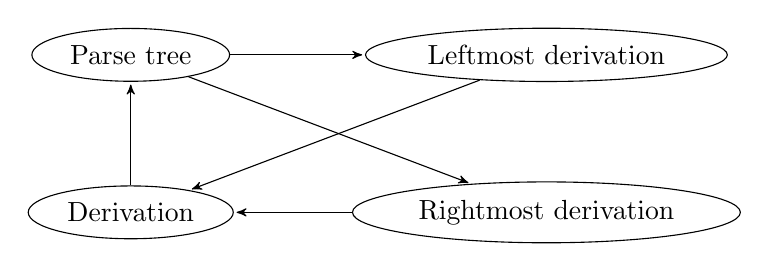
\begin{tikzpicture}						
				\node[elliptic state] (q0)      {Derivation};
				\node[elliptic state] (q01)  [right=1.5cm of q0]     {Rightmost derivation};
				\node[elliptic state] (q02)  [above of=q01]     {Leftmost derivation};
				\node[elliptic state] (q03)  [above of=q0]     {Parse tree};
				\path[->]
					(q0)  edge  node {} (q03)
					(q01)  edge  node  {} (q0)
					(q02)  edge  node  {} (q0)
					(q03)  edge  node {}  (q01)
					(q03)  edge  node {}  (q02);
			\end{tikzpicture}			
		}
	\end{center}

\end{frame}


\begin{frame}{Parse tree to leftmost derivation: an example}

	\begin{columns}

		\column{0.2\textwidth}

		\vspace{-12pt}
		\begin{center}
			\scalebox{0.9}{
				\begin{forest}
				[E [E [I [a]]] [*][E[(][E[E[I [a]]][+][E[I [I[I[b]][0]][0]]]][)]]]
				\end{forest}
			} 
		\end{center}	
	
		\column{0.8\textwidth}

		\begin{itemize}
			\item Root: $E\Rightarrow_{lm} E*E $
			\item Leftmost child of the root: $E\Rightarrow_{lm}I\Rightarrow_{lm}a$
			\item Rightmost child of the root:
			$E\Rightarrow_{lm}(E) \Rightarrow_{lm}(E+E)\Rightarrow_{lm}(I+E)\Rightarrow_{lm}(a+E)$
			$\Rightarrow_{lm}(a+I)\Rightarrow_{lm}(a+I0)\Rightarrow_{lm}(a+I00)\Rightarrow_{lm}(a+b00) $			
			\item Leftmost integrated to root: $E \Rightarrow_{lm} E*E\Rightarrow_{lm} I*E\Rightarrow_{lm} a*E$
			\item Full derivation: 
			$E \Rightarrow_{lm} E*E\Rightarrow_{lm} I*E\Rightarrow_{lm} a*E\Rightarrow_{lm}$
			$\Rightarrow_{lm}a*(E) \Rightarrow_{lm}a*(E+E)\Rightarrow_{lm}a*(I+E)\Rightarrow_{lm}$
			$\Rightarrow_{lm}a*(a+E)
			\Rightarrow_{lm}a*(a+I)\Rightarrow_{lm}a*(a+I0)\Rightarrow_{lm}$
			$\Rightarrow_{lm}a*(a+I00)\Rightarrow_{lm}a*(a+b00) $
		\end{itemize}
		
	\end{columns}	

\end{frame}


\begin{frame}{Parse tree to leftmost derivation: the proof}

	\textbf{Observe:} If $\beta_1\Rightarrow\beta_2\Rightarrow\dots\Rightarrow\beta_n$ is a derivation, then for any $\alpha,\alpha'\in (V\cup T)^*$, $\alpha\beta_1\alpha'\Rightarrow\alpha\beta_2\alpha'\Rightarrow\dots\Rightarrow\alpha\beta_n\alpha'$ is a derivation.

	Suppose we have a parse tree with root $A$ and yield $\gamma$. Induction on the depth of the tree.

	\textbf{Base:} depth 1, root $A$ with children that read $\gamma$ 
	
	$A\rightarrow\gamma$ is a production, thus $A\Rightarrow_{lm}\gamma$ is a one-step derivation

	\textbf{Induction step:} depth $n>1$, root $A$ with children $X_1,X_2,\dots,X_k$
	
	\begin{itemize}
		\item If $X_i$ is a terminal, define $\gamma_i=X_i$
		\item If $X_i$ is a variable, then by induction $X_i\Rightarrow^*_{lm}\gamma_i$.
	\end{itemize}
	To construct the leftmost derivation, show by induction on $i=1,\dots,k$ that \alert{$A \Rightarrow^*_{lm}\gamma_1\gamma_2\dots \gamma_i X_{i+1}X_{i+2}\dots X_{k}$}

	Finally, when $i=k$, the result is a leftmost derivation of $\gamma$ from $A$.
	
\end{frame}


\begin{frame}{The induction within the induction}

	Assuming that $A \Rightarrow^*_{lm}\gamma_1\gamma_2\dots \gamma_{i-1}X_iX_{i+1}X_{i+2}\dots X_{k}$, show
	$$
	\alert{A \Rightarrow^*_{lm}\gamma_1\gamma_2\dots \gamma_i X_{i+1}X_{i+2}\dots X_{k}}
	$$

	\begin{itemize}
		\item If $X_i$ is a terminal, do nothing, just increment $i$.
		\item If $X_i$ is a variable, rewrite the derivation
		$$
		X_i\Rightarrow_{lm}\alpha_1\Rightarrow_{lm}\alpha_2 \dots \Rightarrow_{lm}\gamma_i
		$$
		to the following:
		\begin{align*}
			\gamma_1\gamma_2\dots \gamma_{i-1}X_iX_{i+1}X_{i+2}\dots X_{k}&\Rightarrow_{lm} \\
			\gamma_1\gamma_2\dots \gamma_{i-1}\alpha_1 X_{i+1}X_{i+2}\dots X_{k}&\Rightarrow_{lm} \\
			\vdots&\\
			\Rightarrow_{lm}\gamma_1\gamma_2\dots \gamma_{i-1}\gamma_iX_{i+1}X_{i+2}\dots X_{k}&
		\end{align*}
	\end{itemize}

	\bigskip

	(To construct a rightmost derivation, go from $i=k$ down to $1$.)

\end{frame}


\begin{frame}{Derivation to parse tree}

	Suppose we have a derivation $A=\beta_1\Rightarrow\beta_2\Rightarrow\dots\Rightarrow\beta_n=\gamma$. 
	
	We construct a parse tree with root $A$ and yield $\gamma$ by induction on the number of steps $n$ in the derivation.

	\textbf{Base} ($n=1$)\textbf{:} $A$ is a single-vertex parse tree

	\textbf{Induction step} ($n>1$) \textbf{:} We have $A\Rightarrow^*\beta_{n-1}\Rightarrow\beta_n$. 
	
	Suppose $\beta_{n-1}=\alpha C\alpha'$ and $\beta_n=\alpha\delta\alpha'$ for a production $C\to\delta$.


	By induction, we have a parse tree with root $A$ and yield $\alpha C\alpha'$. Find the leaf corresponding to $C$ and append to it new leaves labelled by the symbols from $\delta$.
	
	\bigskip

	This shows that (i)$\Rightarrow$(iv), and thus the theorem is proved. \hfill\qedsymbol
	
\end{frame}


\section{2.5 Ambiguity in grammars}


\begin{frame}{Ambiguity: an example}	

	\bigskip
	\begin{tabular}{c c c}
		$E\Rightarrow E+E\Rightarrow E+E*E$ & \hspace{1em} &
		$E\Rightarrow E*E\Rightarrow E+E*E$ \\
		\begin{forest} 
		[E [E][+][E[E][*][E]]]
		\end{forest}
		& &
		\begin{forest} 
		[E[E[E][+][E]][*][E]]
		%\node at (current bounding box.south) [below=1ex] {2.derivation}; 
		\end{forest}
	\end{tabular}
	\begin{itemize}
		\item \alert{Two different parse trees for the same expression.}
		\item Important difference: $1+(2*3)=7 $ but $(1+2)*3=9$
		\item Imagine source file interpretable as two different programs.
		\item This grammar can be modified to remove ambiguity.
		\item Different derivations with the same parse tree are not an issue (e.g. left-most and right-most).
	\end{itemize}

\end{frame}


\begin{frame}{Amiguous context-free grammars}

	A context-free grammar $G$ is \alert{ambiguous} if for some $\omega\in L(G)$ there exist two different parse trees with root $S$ and yield~$\omega$. Otherwise the grammar is \alert{unambiguous}.
	
	\bigskip

	\textbf{Example:} our grammar for simple expressions is ambiguous, $\omega=a+a*a\in L(G)$ is yielded by both of the following parse trees:

	\begin{center}
		\scalebox{0.8}{
			\begin{forest} 
				[E [E[I[a]]][+][E[E[I[a]]][*][E[I[a]]]]]
			\end{forest}\hspace{1cm}
			\begin{forest} 
				[E[E[E[I[a]]][+][E[I[a]]]][*][E[I[a]]]]	
			\end{forest}		
		}
	\end{center}	

\end{frame}


\begin{frame}{Inherent ambiguity of context-free languages}
	
	A context-free language $L$ is \alert{unambiguous} if there exists an unambiguous grammar generating it, and $L$ is \alert{inherently ambiguous} otherwise (i.e., if every CFG for $L$ is ambiguous).

	\smallskip
		
	\textbf{Example:} $L=\{a^nb^nc^kd^k \mid n,k\geq 1\}\cup \{a^nb^kc^kd^n \mid n,k\geq 1\}$ is inherently ambiguous. Here is an ambiguous grammar with two parse trees for $\omega=aabbccdd$.

	\begin{multicols}{3}
		
		$S\rightarrow  AB\mid C$\\
		$A\rightarrow  aAb\mid ab$\\
		$B\rightarrow  cBd\mid cd$\\
		$C\rightarrow  aCd\mid aDd$\\
		$D\rightarrow  bDc\mid bc$
				
		\begin{center}
			\scalebox{0.6}{
				\begin{forest}
					[S[A [a][A[a][b]][b]] [B [c][B[c][d]][d]]]
				\end{forest}
			}
		\end{center}

		\begin{center}
			\scalebox{0.6}{
				\begin{forest}
					[S[C[a][C[a][C[b][D[D[b][c]]][c]][d]][d]]]
				\end{forest}
			}
		\end{center}		

	\end{multicols}

	\vspace{-2cm}
	Why \alert{inherently}? Idea: any grammar will generate\\ at least some $a^nb^nc^nd^n$ in the two different ways.

\end{frame}


\begin{frame}{Removing ambiguity}

	\begin{itemize}
		\item There is no algorithm deciding if a given CFG is ambiguous.
		\item There exist inherently ambiguous context-free languages (see the example above).
		\item There are certain techniques for removing ambiguity.
	\end{itemize}

	Different causes for ambiguity:
	\begin{itemize}
		\item The precedence of operators is not respected.
		\item A sequence of identical operators associates from left or right.
		\item E.g. for rules $S\rightarrow\ \mathtt{if}\ \mathtt{then}\ S\ \mathtt{else}\ S\mid\ \mathtt{if}\ \mathtt{then}\ S\mid\epsilon$, the word \alert{\texttt{if then if then else}} has two meanings:
		\alert{\texttt{if then (if then else)}} or \alert{\texttt{if then (if then) else}}

		\medskip
		Possible solutions:
		\begin{itemize}
			\item syntax error (Algol 60)
			\item \texttt{else} belongs to the closer \texttt{if} (rules ordered by preference)
			\item parentheses, \texttt{begin}---\texttt{end}, or indentation (Python)
		\end{itemize}
	\end{itemize}

\end{frame}


\begin{frame}{Enforcing precedence}

	Introduce a new variable for each level of `binding strength':
`	\begin{itemize}
		\item a \alert{factor} is an expression that cannot be broken by any operator: identifiers, parenthesized expressions
		\item a \alert{term} is an expression not broken by $+$
		\item an \alert{expression} can be broken by either $*$ or $+$.
	\end{itemize}
	
	\begin{columns}

		\column{0.6\textwidth}

		An unambiguous grammar:

		\bigskip
		
		$I\rightarrow  a\mid  b\mid Ia\mid Ib\mid I0\mid I1$\\
		$F\rightarrow  I\mid (E) $\\
		$T\rightarrow  F\mid T*F $\\
		$E\rightarrow  T\mid E+T $

		\bigskip

		right: the only parse tree for $a+a*a$
			
		\column{0.4\textwidth}
		
		\begin{center}
			\scalebox{0.8}{
				\begin{forest}
					[E [E[T[F[I[a]]]]][+][T[T[F[I[a]]]][*][F[I[a]]]]]
				\end{forest}
			}
		\end{center}
				
	\end{columns}

\end{frame}


\begin{frame}{Unambiguity and compilers}

	Compiling an expression (a stack for intermediate results + two registers):
	
	\begin{tabular}{c l l}
		(1) &$E\rightarrow  E+T $ & ... \texttt{pop r1; pop r2; add r1,r2; push r2}\\
		(2) &$E\rightarrow  T $ & \\
		(3) &$T\rightarrow  T*F $& ... \texttt{pop r1; pop r2; mul r1,r2; push r2}\\
		(4) &$T\rightarrow  F $& \\
		(5) &$F\rightarrow (E) $& \\
		(6) &$F\rightarrow a $& ... \texttt{push a}
	\end{tabular}

	\begin{itemize}
		\item `a+a*a' is obtained by applying rules 1,2,4,6,3,4,6,6
		\item reverse the sequence and choose only code-generating rules:
		
		6,6,3,6,1

		\item now replace the rules with the corresponding code:
		
		\texttt{push a; push a; pop r1; pop r2; mul r1,r2; push r2; push a; pop r1; pop r2; add r1,r2; push r2} 
	\end{itemize}

\end{frame}


\begin{frame}{Summary of Lecture 5}
	
	\begin{itemize}
		\item Grammars: general, context-sensitive, context-free, right-linear (regular) -- Chomsky hierarchy
		\item The language of a grammar, derivation
		\item Right-linear grammars correspond to FA (and so do left/linear)
		\item Linear grammars are stronger
		\item Context-free grammars: parse tree and its yield
		\item (un)ambiguous grammars, inherently ambiguous languages
	\end{itemize}

\end{frame}


\end{document}
